\documentclass[a4paper,article,14pt]{extarticle}

\usepackage{spbudiploma}
\usepackage{amsmath}
\usepackage{mathtools}
\usepackage[pdftex]{graphicx}
\graphicspath{{../pictures/}}
\usepackage{listings}
\usepackage{xcolor}

\definecolor{codegreen}{rgb}{0,0.6,0}
\definecolor{codegray}{rgb}{0.5,0.5,0.5}
\definecolor{codepurple}{rgb}{0.58,0,0.82}
\definecolor{backcolour}{rgb}{0.95,0.95,0.92}

\lstdefinestyle{mystyle}{
	backgroundcolor=\color{backcolour},   
	commentstyle=\color{codegreen},
	keywordstyle=\color{codegreen},
	numberstyle=\tiny\color{codegray},
	stringstyle=\color{codepurple},
	basicstyle=\ttfamily\footnotesize,
	breakatwhitespace=false,         
	breaklines=true,                 
	captionpos=b,                    
	keepspaces=false,                 
	numbers=left,                    
	numbersep=5pt,                  
	showspaces=false,                
	showstringspaces=false,
	showtabs=false,                  
	tabsize=2
}

\lstset{style=mystyle}

\begin{document}
	\begin{titlepage}
		\begin{center}
			FEDERAL STATE AUTONOMOUS EDUCATIONAL INSTITUTION
			
			OF HIGHER EDUCATION
			
			ITMO UNIVERSITY
			\vspace{3cm}
			
			\large\textbf{Report}
			
			\large on the practical task No.1
			
			\large \flqq Experimental time complexity analysis\frqq
			\vspace{5cm}
			
			
			\begin{flushright}
				{Performed by:} \\
				Putnikov Semyon \\ 
				J4132c \\
			\end{flushright}
			
			
			\begin{flushright}
				{Accepted by:} \\
				Dr Petr Chunaev \\ 
			\end{flushright}
			\vfill
			
			{St.Petersburg}
			\par{\number\year}
		\end{center}
	\end{titlepage}
	
	\newpage
	
	\section{Goal}
	Experimental study of the time complexity of different algorithms.
	
	\section{Formulation of the problem}
	
	For each n from 1 to 2000, measure the average computer execution time (using timestamps) of programs implementing the algorithms and functions below for five runs. Plot the data obtained showing the average execution time as a function of n. Conduct the theoretical analysis of the time complexity of the algorithms in question and compare the empirical and theoretical time complexities.
	
	\begin{enumerate}
		\item Generate an n-dimensional random vector $\vec{v}$ with non-negative elements. For $\vec{v}$  implement the following calculations and algorithms:
		\begin{enumerate}
			\item \begin{math} f(v) = const \end{math} \textit{(constant function)}
			\item \begin{math} f(v) = \sum_{k=1}^n v_k\end{math} \textit{(the sum of elements)}
			\item \begin{math} f(v) = \prod_{k=1}^n v_k\end{math} \textit{(the product of elements)}
			\item supposing that the elements of $\vec{v}$ are the coefficients of a polynomial \textit{P} of degree n-1, calculate the value \textit{P(1.5)} by a direct calculation of $P(x)=\sum_{k=1}^n v_k x^{k-1}$ (i.e. evaluating each term one by one) and by Horner’s method by representing the polynomial as $P(x)=v_1+x(v_2+x(v_3+...))$;
			\item Bubble Sort of the elements of $\vec{v}$;
			\item Quick Sort of the elements of $\vec{v}$;
			\item Timsort of the elements of $\vec{v}$;
		\end{enumerate}
		\item Generate random matrices \textit{A} and \textit{B} of size $n\times n$ with non-negative elements. Find the usual matrix product for \textit{A} and \textit{B}.
		\item Describe the data structures and design techniques used within the algorithms.
	\end{enumerate}
	
	\section{Brief theoretical part}
	\subsection{Horner's method}
	
	Horner's method is a method for approximating the roots of polynomials that was described by William George Horner in 1819.
	
	Given the polynomial $p(x)=\sum_{k=1}^n a_i x^i=a_0+a_1 x+a_2 x^2+a_3 x^3+...+a_n x^n$ where $a_0,...a_n$ are constant coefficients, the problem is to evaluate the polynomial at a specific value $x_0$ of $x$.
	
	For this, a new sequence of constants is defined recursively as follows:
	\begin{align}
	b_n &:= a_n \\
	b_{n-1 } &:= a_{n-1}+b_n x_0 \\
	&\vdotswithin{:=} \notag \\
	b_1 &:= a_1+b_2 x_0\\
	b_0 &:= a_0+b_1x_0
	\end{align}
	
	Then $b_0$ is the value of $p(x_0)$. To see why this works, the polynomial can be written in the form 
	\begin{align}
	p(x)=a_0 +x\Bigg(a_1+x\bigg(a_2+x\Big(a_3+...+x\big(a_{n-1} + xa_n\big)...\Big)\bigg)\Bigg)
	\end{align}
	
	\subsection{Bubble sort}
	
	Bubble sort is a simple sorting algorithm that repeatedly steps through the list, compares adjacent elements and swaps them if they are in the wrong order. The pass through the list is repeated until the list is sorted. The algorithm is named for the way smaller or larger elements "bubble" to the top of the list. Best-case perfomance is $O(n)$ and worst-case is $O(n^2)$.
	\subsection{Quick sort}
	
	Quicksort is a divide-and-conquer algorithm. It works by selecting a 'pivot' element from the array and partitioning the other elements into two sub-arrays, according to whether they are less than or greater than the pivot. The sub-arrays are then sorted recursively. This can be done in-place, requiring small additional amounts of memory to perform the sorting. Best-case perfomance is $O(n)$ (three-way partition and equal keys) and worst-case is $O(n^2)$ (one of the sublists returned by the partitioning routine is of size $n - 1$ and pivot happens to be the smallest or largest element in the list).
	
	\subsection{Timsort}
	
	Timsort is a hybrid stable sorting algorithm, derived from merge sort and insertion sort, designed to perform well on many kinds of real-world data. It was implemented by Tim Peters in 2002 for use in the Python programming language. The algorithm finds subsequences of the data that are already ordered (runs) and uses them to sort the remainder more efficiently. This is done by merging runs until certain criteria are fulfilled. Best-case perfomance is $O(n)$ and worst-case is $O(n\log n)$.
	
	\section{Results}
	%Present the results of solving the assigned problems, including graphs and tables, as well as a brief discussion of the results obtained (at most 4 pages)
	\subsection{Constant function (Task I, subtask a)}
	
	At Figure \ref{constant} we can see execution time of constant function. This plot tends to direct line as expected, but have some outliers. It is a result of cpu overheating which affects execution process.
	
	Nevertheless, the graph proofs that the execution time of constant function does not depend on the number of variables.
	
	\subsection{The sum of elements (Task I, subtask b)}
	
	At Figure \ref{sum} we can see that execution time is similar to constant function. Some outliers, caused by cpu overheating also included, but the main thing is that plot tends to direct line. This happens because of using embedded Python function for elements sum. 
	
	So on practice we have something close to constant complexity, not expected $O(n)$
	
	\subsection{The product of elements (Task I, subtask c)}\label{sub:C}
	
	At Figure \ref{product} we can see that execution time is also similar to constant function. We have same situation, as in \ref{sub:C}. We also use embedded Python function, but for elements product this time. 
	On practice we have time complexity, which is close to constant, instead of expected $O(n)$.
	
	\subsection{Polynomial calculation (Task I, subtask d)}
	
	\textit{Direct way.} At Figure \ref{direct} we can see that time complexity is $O(n)$. Theoretically it should be $O(n^2)$, but implementation has no simple loop for evaluation of $x$, it uses embedded programming language function.
	
	
	\textit{Horner's method.} At Figure \ref{horners} plot shows us that time complexity is $O(n)$. This is just as we expected theoretically. Methods includes result initialization as coefficient of $x^n$, repeatedly result with x multiplication and adding next coefficient to result. Finally we return result. 
	
	So we have $O(n)$ both theoretically and on practice. 
	
	\subsection{Bubble Sort (Task I, subtask e)}
	
	At Figure \ref{bubble} we see, that time on plot increases closely to $O(n^2)$. This complexity is theoretically expected, because we have to make $O(n^2)$ comparisons.
	
	\subsection{Quick Sort (Task I, subtask f)}
	
	At Figure \ref{quick} we see, that time on plot increases closely to $O(n\log n)$. This time complexity is average theoretical perfomance, so our practical result completely matches it (excluding cpu-caused outliers).
	
	\subsection{Tim Sort (Task I, subtask g)}
	
	At Figure \ref{tim} we see, that time on plot, as in previous case, increases closely to $O(n\log n)$. This time complexity is also known as average theoretical for this algorithm, so our practical result matches it.
	
	\subsection{Matrices product (Task II)}
	
	Despite all cpu outliers the plot at Figure \ref{matrices} clearly shows us, that time complexity for matrices multiplication is $O(n^3)$. This time complexity matches theoretical one for this algorithm, so our practical result proves it.
	
	\subsection{Data structures and design techniques (Task III)}
	
	We use embedded Python data structures at programming realization of above described algorithms, such as dictionaries and lists. Also it was very helpful to use Dataframe structure from \flqq pandas\frqq $ $ library.
	
	For measuring execution time we use method from library \flqq timeit\frqq. We use library \flqq matplotlib\frqq $ $ to create plots.
	
	As design technique we use pattern decorator and recursive architecture.
	
	
	\section{Conclusions}
	To sum it up, we've measured the average execution time of well-known algorithm implementations, using data plots, representing our time values as a function of n. 
	
	After comparison of the empirical and theoretical time complexities we can say, that sometimes features of programming language helps us to speed up calculations. But also sometimes hardware makes it's adjustments, so we don't have stable time complexity on practice, only approximated values. 
	
	\newpage
	\section{Figures}
	\begin{figure}[h]
		\centering
		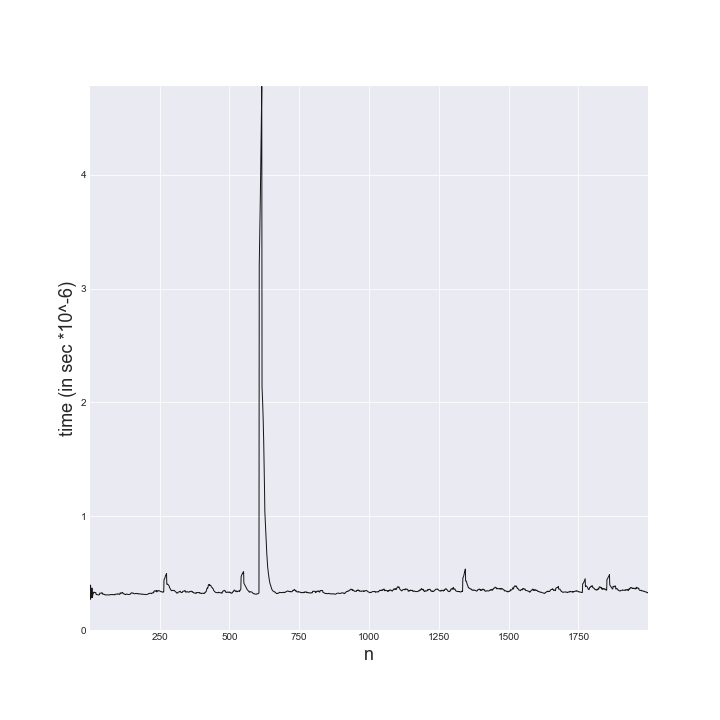
\includegraphics[scale=0.5]{constant.png}
		\caption{Plot of constant function.}
		\label{constant}
	\end{figure} 
	\begin{figure}[h]
		\centering
		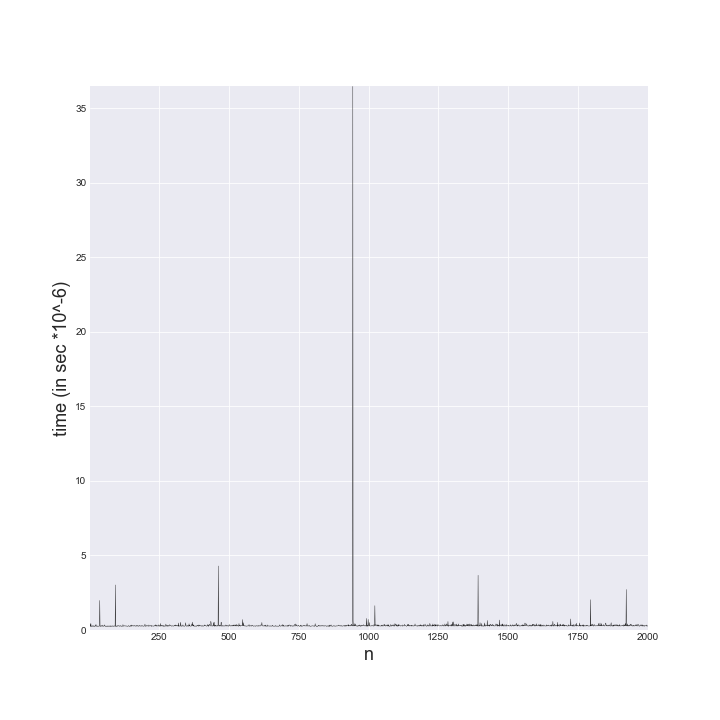
\includegraphics[scale=0.5]{sumOfVector.png}
		\caption{Plot for sum of elements.}
		\label{sum}
	\end{figure} 
	\begin{figure}[h]
		\centering
		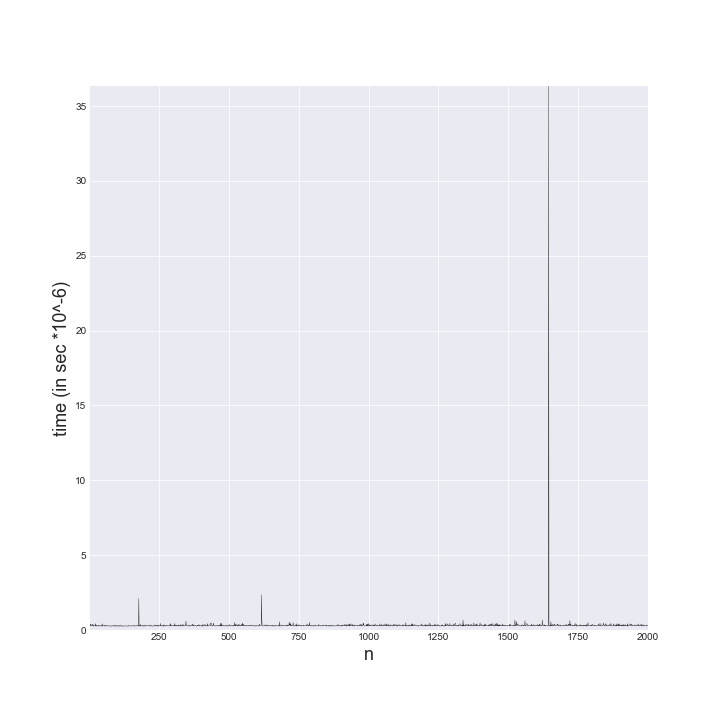
\includegraphics[scale=0.5]{productOfVector.png}
		\caption{Plot for product of elements.}
		\label{product}
	\end{figure} 
	\begin{figure}[h]
		\centering
		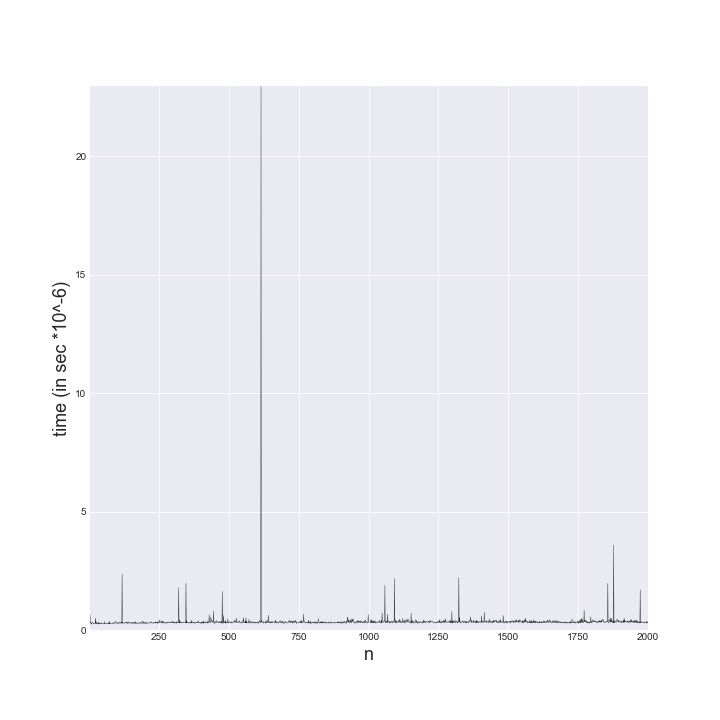
\includegraphics[scale=0.5]{calculatePolinom.png}
		\caption{Plot for direct polynomial calculation.}
		\label{direct}
	\end{figure} 
	\begin{figure}[h]
		\centering
		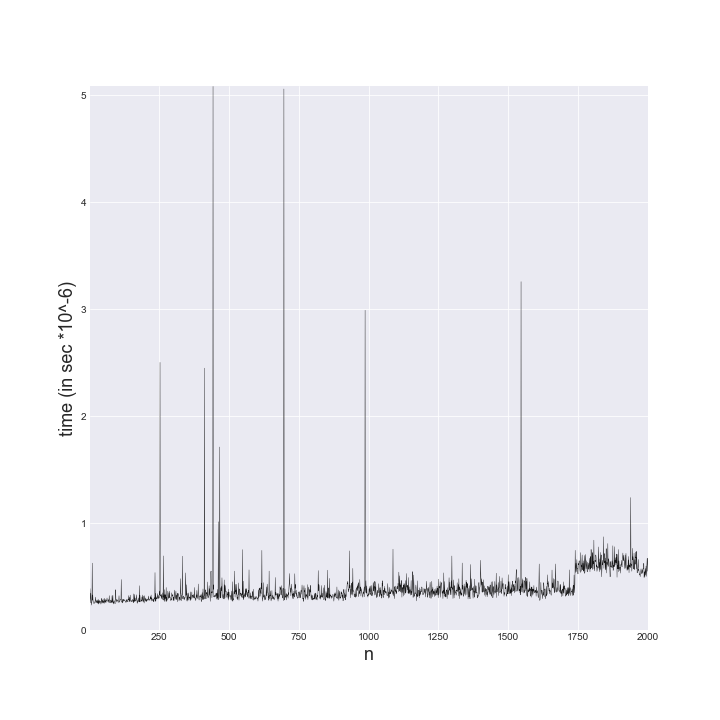
\includegraphics[scale=0.5]{horners.png}
		\caption{Plot for polynomial calculation by Horner's method.}
		\label{horners}
	\end{figure} 
	\begin{figure}[h]
		\centering
		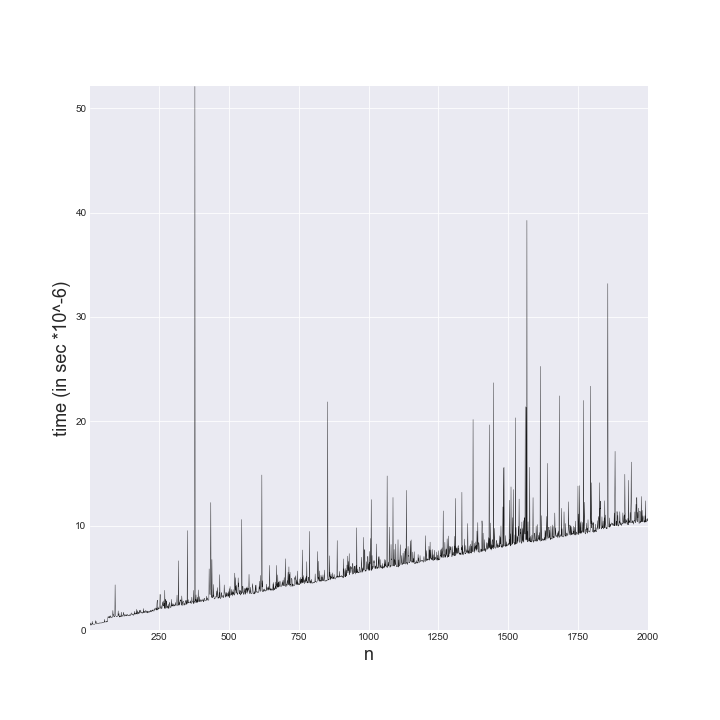
\includegraphics[scale=0.5]{bubbleSort.png}
		\caption{Plot for "bubble" sorting.}
		\label{bubble}
	\end{figure} 
	\begin{figure}[h]
		\centering
		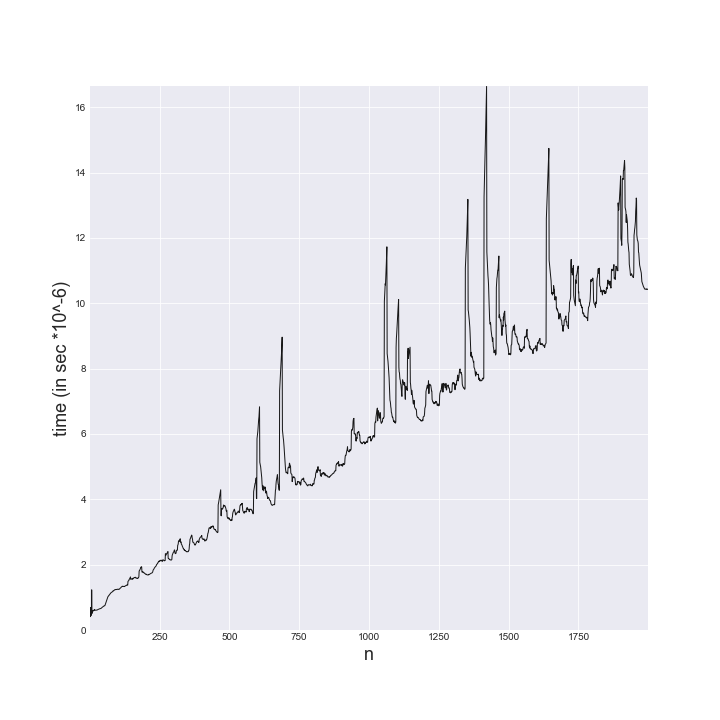
\includegraphics[scale=0.5]{quickSort.png}
		\caption{Plot for "quick" sorting.}
		\label{quick}
	\end{figure} 
	\begin{figure}[h]
		\centering
		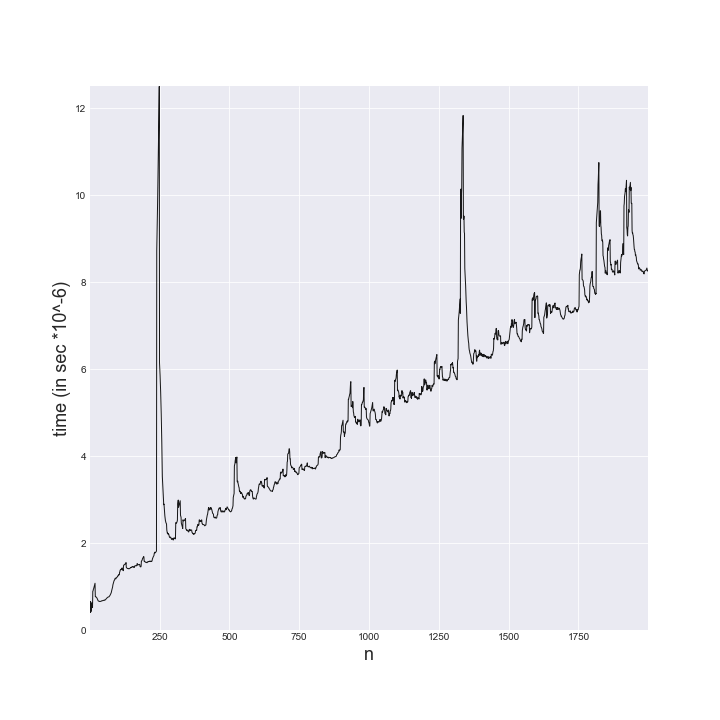
\includegraphics[scale=0.5]{timSort.png}
		\caption{Plot for "Tim" sorting.}
		\label{tim}
	\end{figure} 
	\begin{figure}[h]
		\centering
		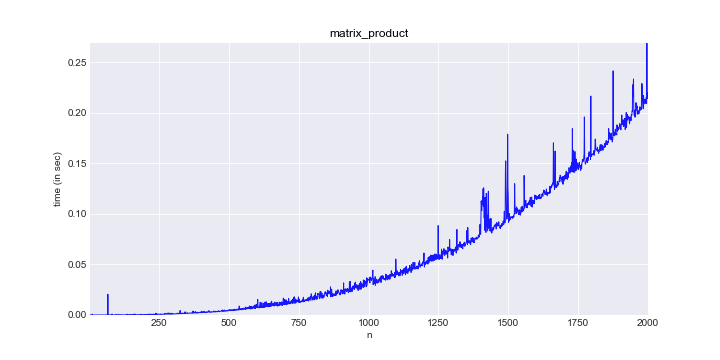
\includegraphics[scale=0.5]{matrix.png}
		\caption{Plot for product of two random matrix.}
		\label{matrices}
	\end{figure}
	
\end{document}